Parasitic computing\footnote{In this thesis we are not covering, neither
we are interested in, the ethical or moral implication of using this technique.}
is a technique that, using some exploits and ad-hoc code, allows a \emph{malicious}
user to use the computational power of the \emph{victim} computer without this
being aware. As one can notice parasitic computing has a strong relationship
with \emph{distributed computing}. In fact is a specialization of the general
class of \emph{distributed computing}, where the user is unaware of
the execution\footnote{In \emph{distributed computing} the user can be unaware
of the actual code they are executing, but they are aware of the execution.}.\\

This approach was first proposed by \cite{barabasi2001parasitic} to solve the
NP-complete 3-SAT problem using the existing TCP/IP protocol stack and its error
handling routines. The satisfiability problems or "SAT" involve finding a
solution to a boolean equation that satisfies a number of logical clauses. For
example, $(x_1 \oplus x_2) \land (x_2 \land x_3 )$ in principle has $2^3$ potential
solutions, but it is satisfied only by the solution: $x_1=1, x_2=0, x_3=1$.
Problems like the one in the example are known as 2-SAT problems because
each clause, shown in parentheses, involves two variables. The more difficult
3-SAT problem is known to be NP-complete, which in practice means that there is
no known polynomial-time algorithm which solves it.\\
\begin{figure}[htb]
    \centering
    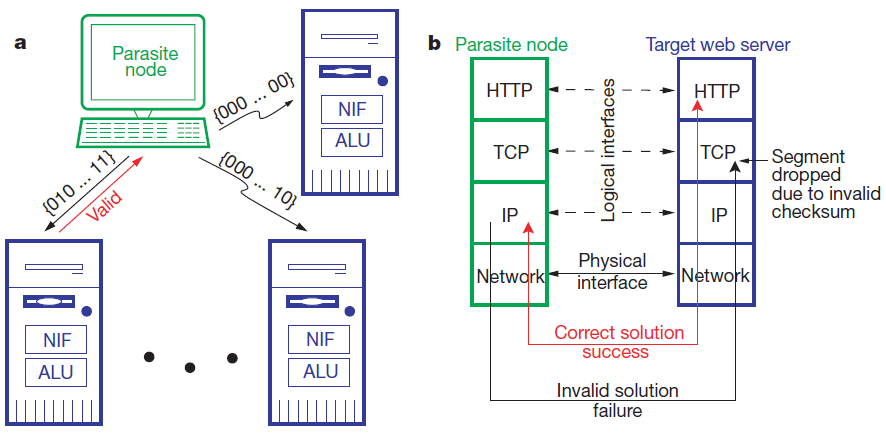
\includegraphics[width=\columnwidth]{parasitic}
    \caption{Schematic diagram of the parasitic computer solving the 3-SAT
    problem.}
    \label{fig:parasitic}
\end{figure}

The approach proposed in the paper was to perform a brute force attack to guess
the right solution of a 3-SAT problem using a parallel approach as depicted in
\autoref{fig:parasitic}. The parasite node creates $2^n$ specially constructed
messages designed to evaluate a potential solution. These messages are sent to
many target servers throughout the Internet. After receiving the message, the
target server verifies the data integrity of the TCP segment by calculating a
TCP checksum. The construction of the message ensures that the TCP checksum fails
for all messages containing an invalid solution to the posed SAT problem. Thus,
a message that passes the TCP checksum contains a correct solution. The target
server will respond to each message it receives (even if it does not understand
the request). As a result, all messages containing invalid solutions are dropped
in the TCP layer. Only a message which encodes a valid solution \emph{reaches}
the target server, which sends a response to the \emph{request} it received.\\

This approach may seem unfair to the user, but
if one thinks about it, may notice how we are always making computation without even
knowing it. \ac{GWAP} or application like \href{http://www.google.com/recaptcha}{reCAPTCHA}
are examples of involuntary human computation (as in \autoref{tab:matrix}). So
they are using the same technique to perform a sort of \emph{parasitic human
computing} without complaining about the users will.\\

A hybrid approach (parasitic \& voluntary) can be used to avoid the ethic implication
of doing pure \emph{Parasitic Computing}. If the user gives the permission to
run computation on its computer exchange of some sort of return, then we are
able to score the best on both approaches. A similar solution was proposed in
\cite{karame2011pay}.
In this paper the authors propose a micro-computation as micro-payments in web-based
services. Their solution is to give the user access to online contents (such as
newspaper, video, etc.) after performing small \js{} computation.

\paragraph{Parasitic \js{}} described in \cite{jenkin2008parasitic} can be
considered as an enhancement of the solution proposed by \cite{barabasi2001parasitic}.
Since using \js{} and the HTML5 features to their full potential (see
\ref{sec:bg:web:html5}) we are able to perform any kind of computation
within the browser window/tab. \js{} offers also a standard platform for the
execution of code without the need of any ad-hoc software for each platform.
Furthermore all the code executed by a browser run in a sandboxed environment,
keeping the user's computer safe from any malicious intent.